\chapter{آزمایش‌ها و نتایج}

\section{دادگان}

\subsection{مجموعه داده \lr{Cityscapes}}

مجموعه داده‌های \verb*|Cityscapes| یکی از پرکاربردترین مجموعه‌های داده برای مسائل تقسیم‌بندی معنایی است، که بر روی درک مفهومی صحنه‌های خیابانی شهری تمرکز دارد. این مجموعه شامل ۵۰۰۰ تصویر با برچسب‌گذاری دقیق و ۲۰۰۰۰ تصویر با برچسب‌گذاری خشن است، که برای ۳۰ کلاس معنایی مختلف آموزش دیده‌اند. تصاویر زیر مقایسه‌ای بین دو نوع برچسب‌گذاری ارائه می‌دهند.

\begin{figure}[ht]
	\centering
	\begin{subfigure}{0.45\textwidth}
		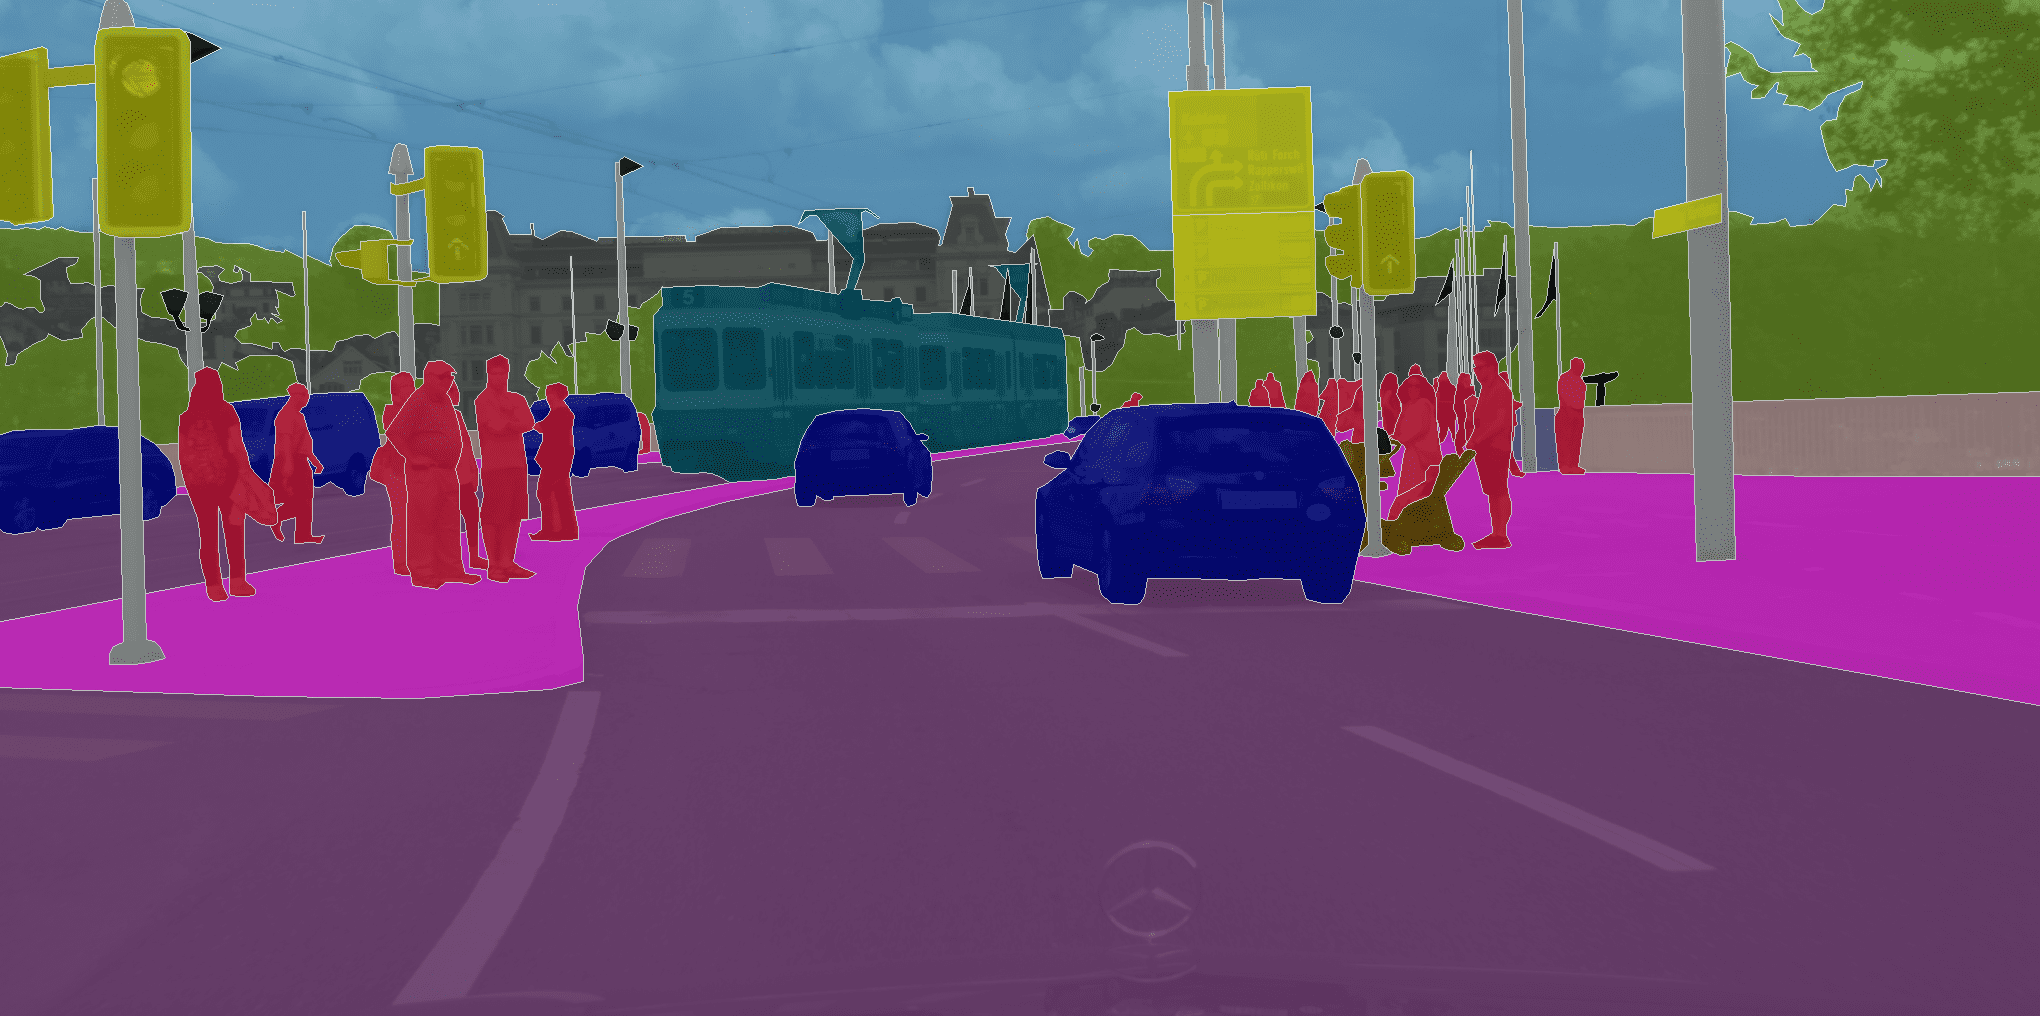
\includegraphics[width=\linewidth, height=0.2\textheight]{Images/Chapter2/Cityscapes/zuerich00.png}
		\caption{برچسب‌گذاری دقیق}
		\label{f64}
	\end{subfigure}\hfil
	\begin{subfigure}{0.45\textwidth}
		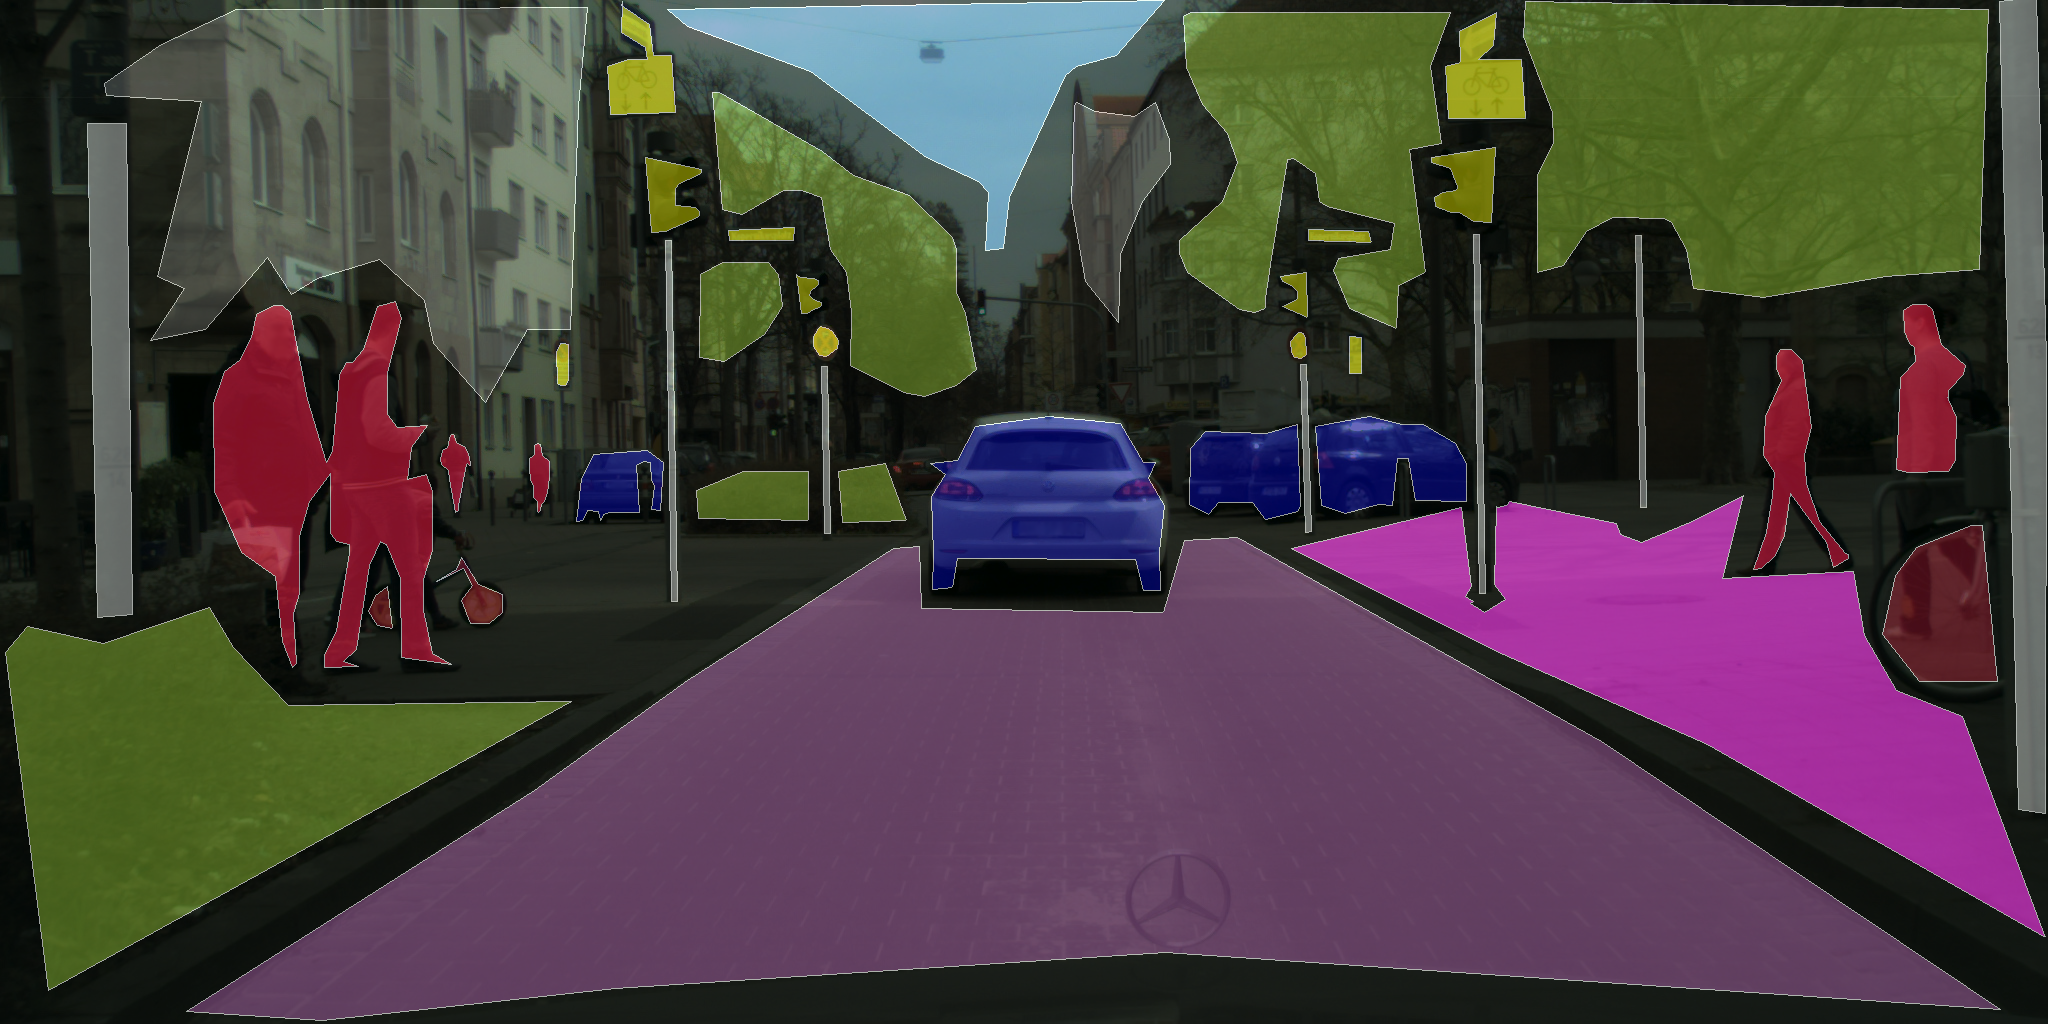
\includegraphics[width=\linewidth, height=0.2\textheight]{Images/Chapter2/Cityscapes/nuremberg00.png}
		\caption{برچسب‌گذاری خشن}
		\label{f65}
	\end{subfigure}
	\caption{انواع بر‌چسب‌گذاری دادگان \lr{Cityscapes}}
	\label{fig:fig1}
\end{figure}

ما در این پژوهش از ۵۰۰۰ تصویر با برچسب‌گذاری شده به شیوه دقیق استفاده خواهیم کرد، چراکه مراجع مورد استفاده قرار گرفته نیز از این نوع برچسب‌گذاری برای مقایسه استفاده کرده اند.

\subsection{مجموعه داده \lr{CamVid}}

در سال ۲۰۰۷، پایگاه داده ویدیویی با برچسب‌گذاری شهری کمبریج (\verb*|CamVid|)، از اولین مجموعه‌های داده تقسیم‌بندی معنایی برای خودروهای خودران، منتشر شد که در آن، ۷۰۰ تصویر از یک دنباله ویدیویی با مدت زمان ۱۰ دقیقه برچسب‌گذاری شد. برای گرفتن ویدیو، دوربین در جلوی ماشین قرار گرفته که دیدگاه مشابهی با راننده دارد. در این مجموعه داده ۳۲ دسته بندی معنایی وجود دارد.

\section{معیار‌های ارزیابی}

\subsubsection{زمان استنتاج}

برای اندازه‌گیری زمان استنتاج از معیار
\verb*|fps|
\LTRfootnote{Frame per second}
استفاده می‌کنیم تا سرعت زمان استنتاج مدل‌ها را با یکدیگر بررسی کنیم. به طبع هر چه
\verb*|fps|
بالاتری داشته باشیم برای ما مطلوب‌تر خواهد بود.


\subsubsection{بهره‌وری منابع}

در این معیار به سه مشخصه زیر می‌پردازیم تا دید بهتری به مقیاس هر مدل پیدا کنیم:

\begin{itemize}
	\item تعداد پارامتر ها: هر چه تعداد نورون‌های بیشتری داشته باشیم مدل سنگین تر می‌شود. تلاش بر آن است که مدل پیشنهادی سبک‌وزن (\lr{lightweight}) باشد.
	\item میزان مصرف مموری: متناسب با پیچیدگی مدل در تعداد و نوع عملیات‌ها میزان مصرف مموری در حین اجرا متغیر است.
	\item میزان مصرف حافظه: این مقدار با تعداد پارامتر‌ها نسبت مستقیم دارد، اما دید شهودی به مقیاس هر مدل می‌دهد.
\end{itemize}

\subsubsection{میانگین اشتراک بر اجتماع}

میانگین اشتراک بر اجتماع
\LTRfootnote{Mean intersection-over-union (Mean IoU)}
یک معیار پرکاربرد در مسائل بینایی ماشین
\LTRfootnote{Computer vision}
است که برای ارزیابی عملکرد مدل‌ها مورد استفاده قرار می‌گیرد و به وسیله محاسبه میزان تطابق بین ماسک تشخیص
\LTRfootnote{Prediction mask}
شیء پیش‌بینی شده توسط مدل و ماسک واقعی در تصویر عمل می‌کند. برای محاسبه این معیار، ابتدا
\verb*|IoU|
یا اشتراک بر اجتماع برای هر شیء در تصویر محاسبه می‌شود، سپس از آن‌ها میانگین گرفته می‌شود تا عملکرد کلی مدل در تشخیص شیء مورد ارزیابی قرار گیرد.

در اینجا اشتراک بر اجتماع هر دسته و میانگین کلی به صورت جدا سنجیده و مقایسه می‌شود.

\section{شرایط آزمایش}

برای ایجاد یک مقایسه عادلانه، دادگان مورد استفاده قرار گرفته را به دو بخش مجموعه‌داده آموزشی
\LTRfootnote{Training set}
و مجموعه‌داده صحبت‌سنجی
\LTRfootnote{Validation set}
تقسیم کردیم. تقسیم‌بندی به همانگونه که در دادگان اولیه انجام‌شده بود نگه‌داشته شد تا در مقایسه با مقاله‌های معتبر دچار مشکل نشویم.
تمامی مدل‌های پیاده سازی شده در چهارچوب پیاده‌سازی پایتورچ
\LTRfootnote{PyTorch framework}
پیاده‌سازی شده اند و تمامی آن‌ها بر روی کارت گرافیکی
\lr{NVIDIA GeForce GTX 3060 6GB}
انجام شده است.
\section{نتایج آزمایش و مقایسه}

در ابتدا به بررسی سرعت پردازش (
\verb*|fps|
) پرداخته می‌شود. در آزمایش فرض شده ۱۰ دسته‌بندی اشیاء داشته و تمامی تصاویر دارای ۳ کانال رنگی هستند. به دلیل محدودیت سخت‌افزاری روی پردازنده گرافیکی این مقایسه بر روی تصاویر با ابعاد ۲۰۴۸ در ۱۰۲۴ انجام نشده است. نتایج در جدول زیر قابل مشاهده است.

\begin{table}[ht]
	\centering
	\renewcommand{\arraystretch}{1.5}
	\begin{tabular}{cc|ccccc}
		\hline
		\multicolumn{2}{c|}{کارت گرافیک / ابعاد / مدل} & \lr{FastSCNN} & \lr{SQNet} & \lr{ENet} & \lr{UNet} & \lr{SegNet} \\
		\hline
		\multirow{4}{*}{\lr{RTX 3060}}
			& \lr{64x128}	& $96.18$ & $139.73$ & $38.81$ & $168.74$ & $140.56$ \\
			& \lr{128x256} 	& $100.07$ & $123.07$ & $38.10$ & $130.11$ & $107.96$ \\
			& \lr{256x512} 	& $98.94$ & $63.87$ & $36.02$ & $45.12$ & $39.92$ \\
			& \lr{512x1024} & $97.93$ & $21.94$ & $30.75$  & $13.71$  & $11.91$ \\
		\hline
		\multirow{5}{*}{\lr{Tesla P100}}
			& \lr{64x128}	& $191.52$ & $304.96$ & $78.32$ & $344.32$ & $284.59$ \\
			& \lr{128x256}  & $189.04$ & $231.09$ & $76.47$ & $211.73$ & $169.51$ \\
			& \lr{256x512}  & $186.67$ & $102.30$ & $76.70$ & $73.58$ & $63.64$ \\
			& \lr{512x1024} & $182.83$ & $34.52$ & $60.25$ & $21.36$ & $18.65$ \\
			& \lr{1024x2048}& $172.34$ & $8.79$ & $24.25$ & $5.46$ & $4.67$ \\
		\hline
	\end{tabular}
	\caption{مقایسه شاخص \lr{fps} روی کارت گرافیکی‌های متفاوت}
	\label{Table1}
\end{table}

با مقایسه نتایج جدول
\ref{Table1}
می‌توان مشاهده می‌شود مدل
\verb*|FastSCNN|
بر روی تصاویر با ابعاد بزرگ بهتر از مدل‌های دیگر عمل می‌کند و مدل
\verb*|SQNet|
برای تصاویر کوچک‌تر بهت عمل می‌کند. علت نتایج متفاوت به ضعیف‌تر نسبت به مقادیر ارائه شده در مقاله‌های اصلی، کارت گرافیکی متفاوت (و ضعیف‌تر) استفاده شده و تفاوت‌هایی در پیاده‌سازی‌های صورت گرفته است. این تفاوت‌ها در مقایسه تعداد پارامتر‌های مدل‌های پیاده‌سازی شده که در جدول
\ref{Table2}
قابل مشاهده است مشهود است. شکل زیر نمایش بهتری از روند تغییر فریم بر ثانیه نشان می‌دهد:

\begin{figure}[ht]
	\centering
	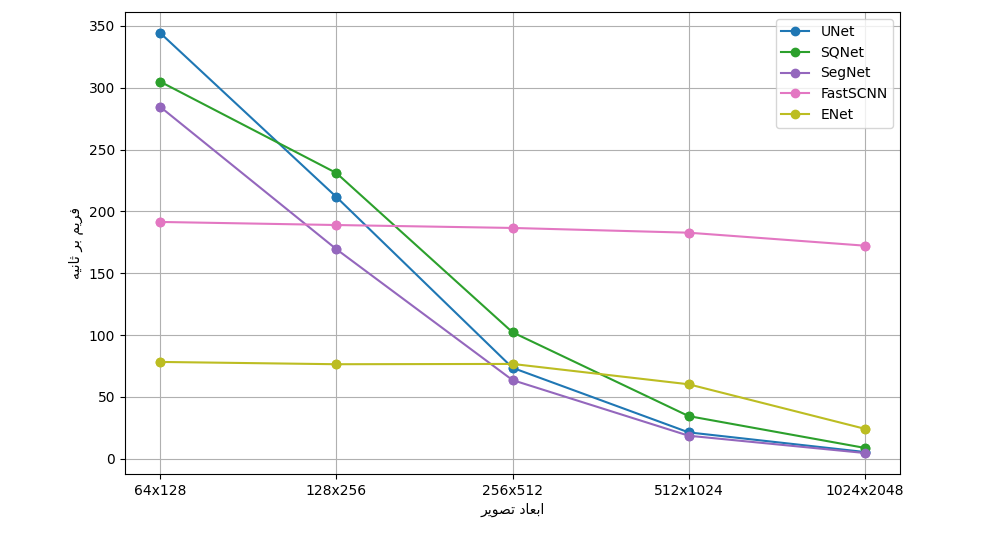
\includegraphics[width=\linewidth, height=0.4\textheight]{Images/Chapter4/FPS_Pattern.png}
	\caption{روند تغییر \lr{FPS} بر حسب افزایش ابعاد تصویر}
	\label{fig:fig11}
\end{figure}

در گام بعد، میزان منابع مورد نیاز برای اجرای مدل‌های معرفی شده برای تصاویر رنگی با ابعاد ۲۵۶ در ۵۱۲ پیکسل بر روی ۱۰ دسته‌ بررسی می‌شود. همانطور که مشخص شده مدل
\verb*|FastSCNN|
از بقیه مدل‌ها سبک‌تر بوده و کاندید مناسب‌تری برای استفاده در سامانه‌های نهفته
\LTRfootnote{Embedded systems}
است.

\begin{table}[ht]
	\centering
	\renewcommand{\arraystretch}{1.5}
	\begin{tabular}{|l|c|c|}
		\hline
		مدل / شاخص & تعداد پارامتر ها (میلیون) & اندازه مدل (گیگابایت) \\ \hline
		\lr{FastSCNN} 	& $1.14$ & $0.21$ \\  \hline
		\lr{SQNet}		& $16.25$ & $0.53$ \\  \hline
		\lr{ENet} 		& $0.36$ & $1.17$ \\ \hline
		\lr{UNet} 		& $13.40$ & $1.81$ \\  \hline
		\lr{SegNet} 	& $29.45$ & $1.02$ \\  \hline
	\end{tabular}
	\caption{مقایسه میزان مصرف منابع}
	\label{Table2}
\end{table}

در آخر شاخص میانگین اشتراک بر اجتماع را بر روی دسته‌بندی ها و گروه ها محاسبه شده است. مجموعه‌داده
\verb*|cityscapes|
دارای ۳۰ دسته و ۷ گروه هست که به طور مستقل شاخص اشتراک بر اجتماع را بر روی آن‌ها محاسبه می‌کنیم.

\begin{table}[ht]
	\centering
	\renewcommand{\arraystretch}{1.5}
	\begin{tabular}{|l|c|c|}
		\hline
		مدل / شاخص & \lr{IoU} دسته & \lr{IoU} گروه \\ \hline
		\lr{FastSCNN} 	& $64.2$ & $78.5$ \\  \hline
		\lr{SQNet} 		& $57.5$ & $72.3$ \\  \hline
		\lr{ENet} 		& $56.0$ & $73.9$ \\  \hline
		\lr{UNet} 		& $66.4$ & $80.7$ \\  \hline
		\lr{SegNet} 	& $55.1$ & $72.0$ \\ \hline
	\end{tabular}
	\caption{مقایسه شاخص اشتراک بر اجتماع}
\end{table}

...

\section{خلاصه}

در آزمایش‌های انجام شده برای ارزیابی عملکرد مدل‌های
\verb*|SQNet|
،
\verb*|FastSCNN|
،
\verb*|ENet|
و
\verb*|SegNet|
بر روی مجموعه داده‌های
\verb*|Cityscapes|
برای مسأله تقسیم‌بندی زمینه‌ای در زمینه خودروهای خودران، یافته‌های مهمی به دست آمد. معیارهای ارزیابی استفاده شده شامل تعداد فریم در ثانیه، میانگین اشتراک بر اجتماع هر کلاس و هر دسته، تعداد پارامترها و اندازه کلی مدل بود.

نتایج نشان می‌دهد که مدل
\verb*|FastSCNN|
می‌تواند با تغییر ابعاد تصویر، تعداد فریم‌های پردازش شده در ثانیه را ثابت نگه دارد. این در حالی است که در مدل‌های دیگر با افزایش اندازه تصویر، کاهش چشم‌گیری در این شاخص دیده می‌شود. همچنین، با وجود اینکه
\verb*|FastSCNN|
کمترین تعداد پارامترها را نداشت، به طور کلی حافظه کمتری نسبت به سایر مدل‌های با معماری رمزگذار-رمزگشا داشت و دقت نسبتاً بالایی در شاخص اشتراک بر اجتماع در هر دو کلاس و دسته نشان داد.

در کل، مشاهده شد که معماری‌ دو شاخه‌ای نسبت به معماری رمزگذار-رمزگشا از نظر سرعت و دقت عملکرد بهتری نشان می‌دهد.

